\subsubsection{Administrationsbereich}
\label{sec:Administrationsbereich}

Ein Oberflächenentwurf des Administrationsbereiches wird in folgender Abbildung dargestellt:

\begin{figure}[htb]
\centering
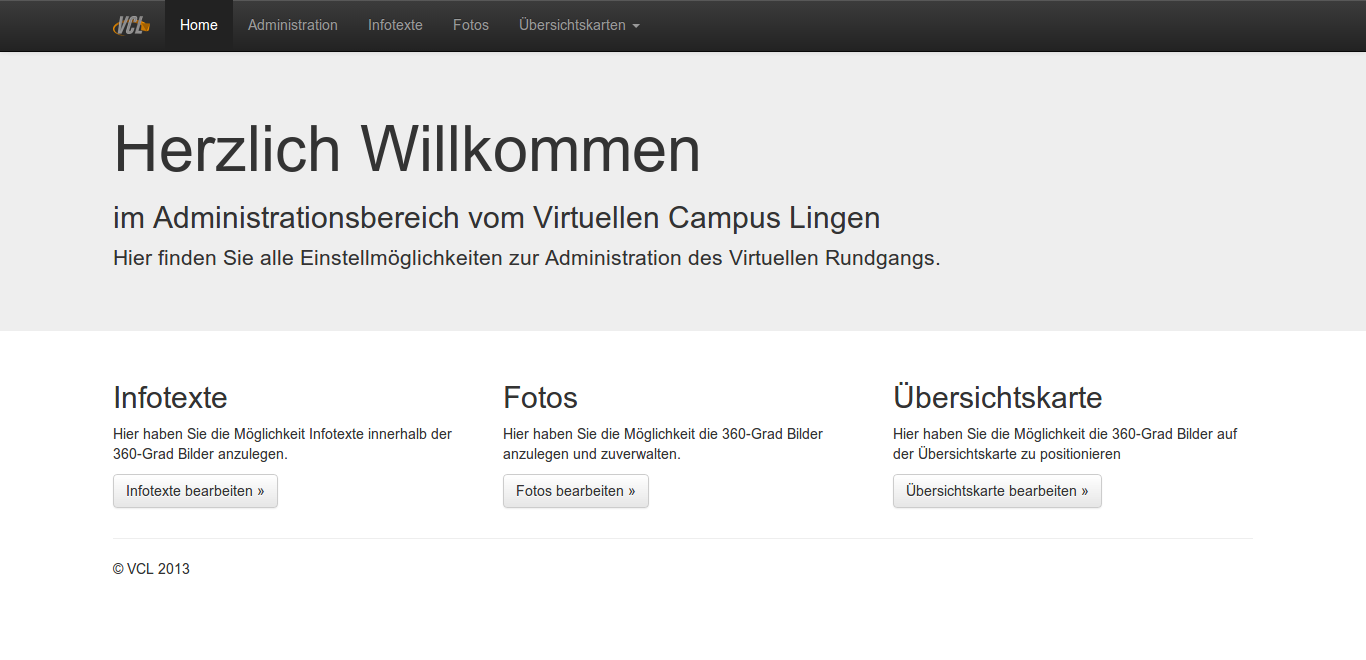
\includegraphics[width=1.0\textwidth]{MockupBackend.png}
\caption[Mockup Backend]{Oberflächenentwurf des
Administrationsbereiches\protect\footnotemark}
\label{fig:MockupBackend}
\end{figure}
\footnotetext{Quelle: Eigene Darstellung}

Der Administrationsbereich ist in vier Bereiche gegliedert:

\begin{itemize}
  \item Infotextverwaltung
  \item Fotoverwaltung
  \item Interessante Ort
  \item Übersichtskarte
\end{itemize}

In der \textbf{Infotextverwaltung} werden Informationstexte geschrieben und zu Panoramafotos zugeordnet. Ein Informationstext kann dabei auch mehreren Fotos zugeordnet werden. Dadurch können dem Benutzer alle Informationstexte angezeigt werden, die sich auf den Auschnitt des Campus beziehen, der gerade betrachtet wird. Alle Informationstexte, die bereits erstellt wurden, werden darüber hinaus tabellarisch angezeigt. Zu jedem angelegten Informationstext gibt es weiterhin die Möglichkeit diesen zu verändern oder zu löschen.

In der \textbf{Fotoverwaltung} werden analog zu der Infotextverwaltung die erstellten Panoramafotos hinterlegt und gepflegt. Erstellte Panoramafotos können in diesem Menüpunkt mit Namen und Beschreibung hochgeladen werden. Analog zu den Infotexten werden auch die bereits hochgeladenen Fotos tabellarisch aufgelistet und mit der Möglichkeit zur Löschung bzw Änderung versehen.

Der Bereich \textbf{Interessante Orte} bietet die Möglichkeit Fotoaufnahmepositionen zu hinterlegen, die dem Benutzer durch Klick auf die Minimap angezeigt werden. Zu diesen Aufnahmepositionen kann der Benutzer dann springen, ohne dorthin navigieren zu müssen. Diese Möglichkeit ist vorallem für Benutzer der Software von Vorteil, die den Campus nicht kennen und nicht erst nach bestimmten Orten (z.B.: Bibliothek) suchen wollen. Zur Pflege dieser Orte muss im entsprechenden Bereich in der Administrationsoberfläche nur ein beschreibender Text eingetragen und mit einem hochgeladenen Foto verlinkt werden.

Die \textbf{Übersichtskarte} stellt den letzen und komplexesten Bereich des Administrationsbereiches dar. In der Übersichtskarte werden die hochgeladenen Panoramafotos auf einer Karte des Hochschulgebäudes platziert. Dazu wird dem angemeldeten Administrator zunächst eine topographische Karte des Campus präsentiert. Auf dieser Karte kann der Administrator durch Klicken eine Position bestimmen, an der ein ausgewähltes Foto gespeichert werden soll.
Ein Foto kann dabei nur an einer Position auf der Übersichtskarte platziert werden. Der Administrator hat die Möglichkeit die Position jedes Fotos beliebig oft zu ändern. Darüber hinaus werden dem Administrator Steuerelemente angezeigt mit denen er einen bestimmten Bereich des Campus auswählen kann, zum Beispiel ein Gebäudetrakt oder ein Stockwerk in einem Gebäudetrakt. Neben der Möglichkeit ein Foto zu positionieren hat der Administrator weiterhin die Möglichkeit
die Verbindung zwischen Fotos pflegen. Aus dem Oberflächenentwurf der Benutzeroberfläche im vorherigen Abschnitt ist ersichtlich, dass ein Benutzer von einem Panoramafoto zu einem anderen navigieren kann. Diese Navigation beruht auf Verbindungen zwischen den Panoramas. Diese Verbindungen werden in der Übersichtskarte geplegt. Die Steuerungselemente des Administrator zu Pflege dieser Verbindungen sind zum Zeitpunkt der Erstellung des Mockups noch nicht definiert, die Notwendigkeit dieser Funktion ist aber bedacht.